\documentclass{assignment}
\ProjectInfos{高等量子力学}{PHYS5001P}{2022-2023 学年第一学期}{第六次作业}{截止时间: 2022 年 10 月 31 日 (周一)}{陈稼霖}[https://github.com/Chen-Jialin]{SA21038052}

\begin{document}
\begin{prob}[课本习题 3.18]
    已知一个在球对称势中的粒子处在 $\bm{L}^2$ 和 $L_z$ 的本征态, 本征值分别为 $l(l+1)\hbar^2$ 和 $m\hbar$. 证明在 $\lvert lm\rangle$ 态之间的期待值满足
    \[
        \langle L_x\rangle=\langle L_y\rangle=0,\qquad\langle L_x^2\rangle=\langle L_y^2\rangle=\frac{[l(l+1)\hbar^2-m^2\hbar^2]}{2},
    \]
    半经典地解释这个结果.
\end{prob}
\begin{pf}
    对 $\lvert lm\rangle$ 态,
    \begin{align}
        \notag\langle L_x\rangle=&\langle lm\rvert L_x\lvert lm\rangle=\langle lm\rvert\frac{L_++L_-}{2}\lvert lm\rangle=\frac{1}{2}(\langle lm\rvert L_+\lvert lm\rangle+\langle lm\rvert L_-\lvert lm\rangle)\\
        \notag=&\frac{1}{2}[\langle lm\rvert\sqrt{(l-m)(l+m+1)}\hbar\lvert l,m+1\rangle+\langle lm\rvert\sqrt{(l+m)(l-m+1)}\hbar\lvert l,m-1\rangle]\\
        =&0,\\
        \notag\langle L_y\rangle=&\langle lm\rvert L_y\lvert lm\rangle=\langle lm\rvert\frac{L_+-L_-}{2i}\lvert lm\rangle=\frac{1}{2i}(\langle lm\rvert L_+\lvert lm\rangle-\langle lm\rvert L_-\lvert lm\rangle)\\
        \notag=&\frac{1}{2i}[\langle lm\rvert\sqrt{(l-m)(l+m+1)}\hbar\lvert l,m+1\rangle+\langle lm\rvert\sqrt{(l+m)(l-m+1)}\hbar\lvert l,m-1\rangle]\\
        =&0,\\
        \notag\langle L_x^2\rangle=&\langle lm\rvert L_x^2\lvert lm\rangle=\langle lm\rvert\left(\frac{L_++L_-}{2}\right)^2\lvert lm\rangle=\frac{1}{4}(\langle lm\rvert L_+^2\lvert lm\rangle+\langle lm\rvert L_+L_-\lvert lm\rangle+\langle lm\rvert L_-L_+\lvert lm\rangle+\langle lm\rvert L_-^2\lvert lm\rangle)\\
        \notag=&\frac{1}{4}[\langle lm\rvert\sqrt{(l-m)(l+m+1)}\hbar\sqrt{(l-m-1)(l+m+2)}\hbar\lvert l,m+2\rangle\\
        \notag&+\langle lm\rvert\sqrt{(l+m)(l-m+1)}\hbar\sqrt{(l-m+1)(l+m)}\hbar\lvert lm\rangle\\
        \notag&+\langle lm\rvert\sqrt{(l-m)(l+m+1)}\hbar\sqrt{(l+m+1)(l-m)}\hbar\lvert lm\rangle\\
        \notag&+\langle lm\rvert\sqrt{(l+m)(l-m+1)}\hbar\sqrt{(l+m-1)(l-m+2)}\hbar\lvert l,m-2\rangle]\\
        =&\frac{[l(l+l)\hbar^2-m^2\hbar^2]}{2},\\
        \notag\langle L_y^2\rangle=&\langle lm\rvert L_y^2\lvert lm\rangle=\langle lm\rvert\left(\frac{L_+-L_-}{2i}\right)\lvert lm\rangle=-\frac{1}{4}(\langle lm\rvert L_+^2\lvert lm\rangle-\langle lm\rvert L_+L_-\lvert lm\rangle-\langle lm\rvert L_-L_+\lvert lm\rangle+\langle lm\rvert L_-^2\lvert lm\rangle)\\
        \notag=&-\frac{1}{4}[\langle lm\rvert\sqrt{(l-m)(l+m+1)}\hbar\sqrt{(l-m-1)(l+m+2)}\hbar\lvert l,m+2\rangle\\
        \notag&-\langle lm\rvert\sqrt{(l+m)(l-m+1)}\hbar\sqrt{(l-m+1)(l+m)}\hbar\lvert lm\rangle\\
        \notag&-\langle lm\rvert\sqrt{(l-m)(l+m+1)}\hbar\sqrt{(l+m+1)(l-m)}\hbar\lvert lm\rangle\\
        \notag&+\langle lm\rvert\sqrt{(l+m)(l-m+1)}\hbar\sqrt{(l+m-1)(l-m+2)}\hbar\lvert l,m-2\rangle]\\
        =&\frac{[l(l+l)\hbar^2-m^2\hbar^2]}{2}.
    \end{align}

    对上述结果的半经典解释: $\lvert lm\rangle$ 为 $\bm{L}^2$ 和 $L_z$ 的共同本征态, $\bm{L}^2\lvert ml\rangle=l(l+1)\hbar^2\lvert lm\rangle$, $L_z\lvert ml\rangle=m\hbar\lvert ml\rangle$, 该本征态关于 $z$ 轴对称, 故角动量的 $L_x$ 和 $L_y$ 分量的均值为零, 此外考虑到经典力学中 $\bm{L}^2=L_x^2+L_y^2+L_z^2$, 故 $\langle L_x^2\rangle=\langle L_y^2\rangle=\frac{1}{2}(\langle\bm{L}^2\rangle-\langle L_z\rangle^2)=\frac{[l(l+1)\hbar^2-m^2\hbar^2]}{2}$.
\end{pf}

\begin{prob}[课本习题 3.20]
    考虑一个轨道角动量的本征态 $\lvert l=2,m=0\rangle$. 假定这个态绕 $y$ 轴转了 $\beta$ 角. 求在 $m=0,\pm 1$ 和 $\pm 2$ 的态上找到这个新态的概率. (在附录 B 的 B.5 节中给出的 $l=0,1$ 和 $2$ 的球谐函数可能是有用的.)
\end{prob}
\begin{sol}
    态 $\lvert l=2,m=0\rangle$ 绕 $y$ 轴转动 $\beta$ 角后变为 $\mathcal{D}(\alpha=0,\beta,\gamma=0)\lvert l=2,m=0\rangle$, 在 $m=0,\pm 1,\pm 2$ 的态上找到这个新态的概率分别为
    \begin{align}
        \notag P(m=0)=&\abs{\langle l=2,m=0\rvert\mathcal{D}^{(l=2)}(\alpha=0,\beta,\gamma=0)\lvert l=2,m=0\rangle}^2=\abs{\mathcal{D}_{00}^{(l=2)}(\alpha=0,\beta,\gamma=0)}^2\\
        \notag=&\abs{\sqrt{\frac{4\pi}{5}}Y_2^{0*}(\beta,0)}^2\\
        =&\frac{1}{4}(3\cos^2\beta-1)^2,\\
        \notag P(m=1)=&\abs{\langle l=2,m=1\rvert\mathcal{D}^{(l=2)}(\alpha=0,\beta,\gamma=0)\lvert l=2,m=0\rangle}^2=\abs{\mathcal{D}_{10}^{(l=2)}(\alpha=0,\beta,\gamma=0)}^2\\
        \notag=&\abs{\sqrt{\frac{4\pi}{5}}Y_2^{1*}(\beta,0)}^2\\
        =&\frac{3}{2}\sin^2\beta\cos^2\beta,\\
        \notag P(m=-1)=&\abs{\langle l=2,m=-1\rvert\mathcal{D}^{(l=2)}(\alpha=0,\beta,\gamma=0)\lvert l=2,m=0\rangle}^2=\abs{\mathcal{D}_{-10}^{(l=2)}(\alpha=0,\beta,\gamma=0)}^2\\
        \notag=&\abs{\sqrt{\frac{4\pi}{5}}Y_2^{-1*}(\beta,0)}^2\\
        =&\frac{3}{2}\sin^2\beta\cos^2\beta,\\
        \notag P(m=2)=&\abs{\langle l=2,m=2\rvert\mathcal{D}^{(l=2)}(\alpha=0,\beta,\gamma=0)\lvert l=2,m=0\rangle}^2=\abs{\mathcal{D}_{20}^{l=2}(\alpha=0,\beta,\gamma=0)}^2\\
        \notag=&\abs{\sqrt{\frac{4\pi}{5}}Y_2^{2*}(\beta,0)}^2\\
        =&\frac{3}{8}\sin^4\theta,\\
        \notag P(m=-2)=&\abs{\langle l=2,m=-2\rvert\mathcal{D}^{(l=2)}(\alpha=0,\beta,\gamma=0)\lvert l=2,m=0\rangle}^2=\abs{\mathcal{D}_{-20}^{l=2}(\alpha=0,\beta,\gamma=0)}^2\\
        \notag=&\abs{\sqrt{\frac{4\pi}{5}}Y_2^{-2*}(\beta,0)}^2\\
        =&\frac{3}{8}\sin^4\theta.
    \end{align}
\end{sol}

\begin{prob}[课本习题 3.24]
    通过把 $j_1=1$ 和 $j_2=1$ 相加, 求出所形成的 $j=2,1,0$ 的所有 $9$ 个 $\lvert j,m\rangle$ 态, 利用简化符号, 以 $\pm,0$ 分别代表 $m_{1,2}=\pm 1,0$. 写出 $\lvert j,m\rangle$ 的显示式, 例如
    \[
        \lvert 1,1\rangle=\frac{1}{\sqrt{2}}\lvert+0\rangle-\frac{1}{\sqrt{2}}\lvert 0+\rangle
    \]
    可以利用阶梯算符 $J_{\pm}$, 或递推关系以及正交性. 找一个克莱布什-戈丹系数表用来做比较, 检验你的结果.
\end{prob}
\begin{sol}
    $j_1=1$ 和 $j_2=1$ 相加所形成的所有 $9$ 个 $\lvert j,m\rangle$ 态分别为
    \begin{gather*}
        \lvert j=2,m=2\rangle,\quad\lvert j=2,m=1\rangle,\quad\lvert j=2,m=0\rangle,\quad\lvert j=2,m=-1\rangle,\quad\lvert j=2,m=-2\rangle,\\
        \lvert j=1,m=1\rangle,\quad\lvert j=1,m=0\rangle,\quad\lvert j=1,m=-1\rangle,\\
        \lvert j=0,m=0\rangle.
    \end{gather*}

    \uline{对于 $j=2$ 的态:} 由于 $m=m_1+m_2$, 易得
    \begin{align}
        \lvert j=2,m=2\rangle=&\lvert++\rangle,\\
        \lvert j=2,m=-2\rangle=&\lvert--\rangle.
    \end{align}
    利用 $J_+=J_{1+}+J_{2+}$ 和 $J_-=J_{1-}+J_{2-}$ 及 $J_{\pm}\lvert jm\rangle=\sqrt{(j\mp m)(j\pm m+1)}\lvert j,m\pm 1\rangle$, $J_{1(2)\pm}\lvert j_{1(2)}m_{1(2)}\rangle=\sqrt{(j_{1(2)}\mp m_{1(2)})(j_{1(2)}\pm m_{1(2)}+1)}\lvert j_{1(2)},m_{1(2)}\pm 1\rangle$, 有
    \begin{gather}
        J_-\lvert j=2,m=2\rangle=2\hbar\lvert j=2,m=1\rangle=(J_{1-}+J_{2-})\lvert++\rangle=\sqrt{2}\hbar\lvert 0+\rangle+\sqrt{2}\hbar\lvert +0\rangle,\\
        \Longrightarrow\lvert j=2,m=1\rangle=\frac{1}{\sqrt{2}}\lvert 0+\rangle+\frac{1}{\sqrt{2}}\lvert+0\rangle,\\
        J_-\lvert j=2,m=1\rangle=\sqrt{6}\hbar\lvert j=2,m=0\rangle=(J_{1-}+J_{2-})\frac{1}{\sqrt{2}}(\lvert 0+\rangle+\lvert+0\rangle)=\lvert-+\rangle+2\lvert 00\rangle+\lvert+-\rangle,\\
        \Longrightarrow\lvert j=2,m=0\rangle=\frac{1}{\sqrt{6}}\lvert-+\rangle+\frac{2}{\sqrt{6}}\lvert 00\rangle+\frac{1}{\sqrt{6}}\lvert+-\rangle,\\
        J_+\lvert j=2,m=-2\rangle=2\hbar\lvert j=2,m=-1\rangle=(J_{1+}+J_{2+})\lvert--\rangle=\sqrt{2}\hbar\lvert 0-\rangle+\sqrt{2}\hbar\lvert-0\rangle,\\
        \Longrightarrow\lvert j=2,m=-1\rangle=\frac{1}{\sqrt{2}}\lvert 0-\rangle+\frac{1}{\sqrt{2}}\lvert-0\rangle.
    \end{gather}

    \uline{对于 $j=1$ 的态:} 由于 $m=m_1+m_2$, 故 $\lvert j=1,m=1\rangle$ 具有 $a\lvert+0\rangle+b\lvert 0+\rangle$ 的形式, 考虑到归一化条件 $\abs{a}^2+\abs{b}^2$ 以及 $\lvert j,m\rangle$ 态之间的正交性, $\lvert j=1,m=1\rangle$ 需与 $\lvert j=2,m=1\rangle=\frac{1}{\sqrt{2}}\lvert 0+\rangle+\frac{1}{\sqrt{2}}\lvert+0\rangle$ 正交, 故必有
    \begin{align}
        \lvert j=1,m=1\rangle=\frac{1}{\sqrt{2}}\lvert+0\rangle-\frac{1}{\sqrt{2}}\lvert 0+\rangle.
    \end{align}
    由此出发, 利用与上面类似的方法有
    \begin{gather}
        J_-\lvert j=1,m=1\rangle=\sqrt{2}\lvert j=1,m=0\rangle=(J_{1-}+J_{2-})\frac{1}{\sqrt{2}}(\lvert+0\rangle-\lvert 0+\rangle)=-\hbar\lvert-+\rangle+\hbar\lvert+-\rangle,\\
        \Longrightarrow\lvert j=1,m=0\rangle=-\frac{1}{\sqrt{2}}\lvert-+\rangle+\frac{1}{\sqrt{2}}\lvert+-\rangle,\\
        J_-\lvert j=1,m=0\rangle=\sqrt{2}\hbar\lvert j=1,m=-1\rangle=(J_{1-}+J_{2-})\frac{1}{\sqrt{2}}(-\lvert-+\rangle+\lvert+-\rangle)=\lvert 0-\rangle-\lvert-0\rangle,\\
        \Longrightarrow\lvert j=1,m=-1\rangle=\frac{1}{\sqrt{2}}\lvert 0-\rangle-\frac{1}{\sqrt{2}}\lvert-0\rangle.
    \end{gather}

    \uline{对于 $\lvert j=0,m=0\rangle$ 态:} 由于 $m=m_1+m_2$, 故 $\lvert j=0,m=0\rangle$ 具有 $\lvert j=0,m=0\rangle=c\lvert+-\rangle+d\lvert 00\rangle+e\lvert-+\rangle$ 的形式, 考虑到归一化条件 $\abs{c}^2+\abs{d}^2+\abs{e}^2=1$ 以及 $\lvert j,m\rangle$ 态之间的正交性,
    \begin{gather}
        \langle j=1,m=0\vert j=0,m=0\rangle=\frac{1}{\sqrt{2}}c-\frac{1}{\sqrt{2}}e=0,\\
        \langle j=2,m=0\vert j=0,m=0\rangle=\frac{1}{\sqrt{6}}c+\frac{2}{\sqrt{6}}d+\frac{1}{\sqrt{6}}e=0,\\
        \Longrightarrow c=\frac{1}{\sqrt{3}},\quad d=-\frac{1}{\sqrt{3}},\quad e=\frac{1}{\sqrt{3}},
    \end{gather}
    故
    \begin{align}
        \lvert j=0,m=0\rangle=\frac{1}{\sqrt{3}}\lvert+-\rangle-\frac{1}{\sqrt{3}}\lvert 00\rangle+\frac{1}{\sqrt{3}}\lvert-+\rangle.
    \end{align}

    上述分解结果与 Clebsch-Gordan 系数表 (图 \ref{6-3-fig}) 一致, 例如, $\lvert j=2,m=1\rangle$ 的展开系数就对应了 $m=1$ 表中 $j=2$ 列的 $\sqrt{\frac{1}{2}},\sqrt{\frac{1}{2}}$.
    \begin{figure}[H]
        \centering
        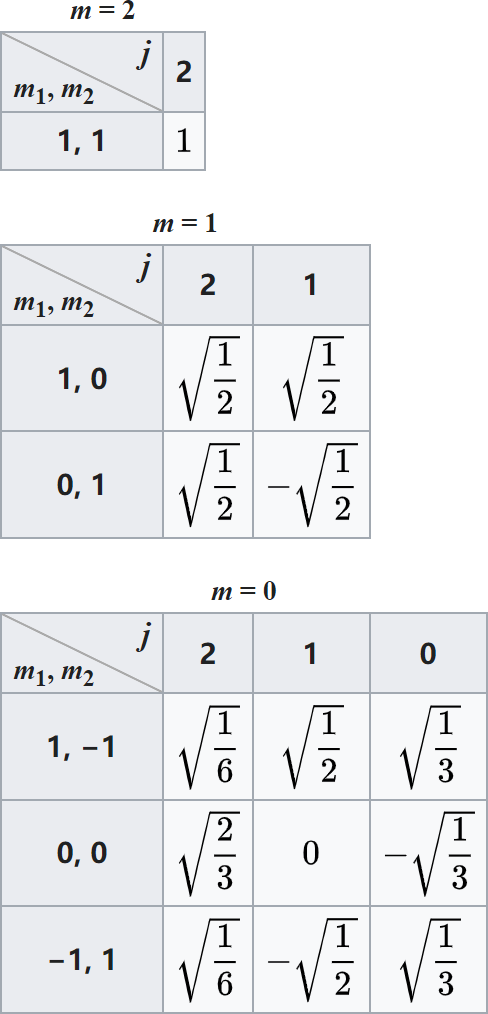
\includegraphics[width=.25\columnwidth]{6-3.png}
        \caption{$j_1=1$ 和 $j_2=1$ 叠加的 Clebsch-Gordan 系数表.}
        \label{6-3-fig}
    \end{figure}
\end{sol}

\begin{prob}[课本习题 3.23]
    在角动量的施温格方案中, 算符
    \[
        K_+\equiv a_+^{\dagger}a_-^{\dagger}\quad\text{和}\quad K_-\equiv a_+a_-
    \]
    的物理意义是什么? 给出 $K_{\pm}$ 的非零矩阵元.
\end{prob}
\begin{sol}
    将 $K_+$ 作用于 $\lvert n_+n_-\rangle$ 上有
    \begin{align}
        K_+\lvert n_+n_-\rangle=a_+^{\dagger}a_-^{\dagger}\lvert n_+n_-\rangle=\sqrt{(n_++1)(n_-+1)}\lvert n_++1,n_-+1\rangle,
    \end{align}
    即 $K_+$ 代表同时产生 (加入) 一个自旋朝上的粒子和一个自旋朝下的粒子, 在 $K_+$ 作用下系统的 $j=\frac{n_++n_-}{2}$ 变为 $j+1=\frac{(n_++1)+(n_-+1)}{2}$, 但角动量的 $z$ 分量 $m=\frac{n_+-n_-}{2}=\frac{(n_++1)-(n_-+1)}{2}$ 不变. $K_+$ 的矩阵元
    \begin{align}
        \notag\langle j'm'\rvert K_+\lvert jm\rangle=&\langle n_+'=j'+m',n_-'=j'-m'\rvert K_+\lvert n_+=j+m,n_-=j-m\rangle\\
        \notag=&\langle n_+'=j'+m',n_-'=j'-m'\rvert\sqrt{(n_++1)(n_-+1)}\lvert n_+=j+m+1,n_-=j-m+1\rangle\\
        \notag=&\langle j'm'\rvert\sqrt{(j+m+1)(j-m+1)}\lvert j+1,m\rangle\\
        =&\sqrt{(j+m+1)(j-m+1)}\delta_{j',j+1}\delta_{m'm}.
    \end{align}

    类似地, 将 $K_-$ 作用于 $\lvert n_+n_-\rangle$ 上有
    \begin{align}
        K_-\lvert n_+n_-\rangle=a_+a_-\lvert n_+n_-\rangle=\sqrt{n_+n_-}\lvert n_+-1,n_--1\rangle,
    \end{align}
    即 $K_-$ 代表同时湮灭 (拿走) 一个自旋朝上的粒子和一个自旋朝下的粒子, 在 $K_-$ 作用下系统的 $j=\frac{n_++n_-}{2}$ 变为 $j-1=\frac{(n_+-1)+(n_--1)}{2}$, 但角动量的 $z$ 分量 $m=\frac{n_+-n_-}{2}=\frac{(n_+-1)-(n_--1)}{2}$ 不变. $K_-$ 的矩阵元
    \begin{align}
        \notag\langle j'm'\rvert K_-\lvert jm\rangle=&\langle n_+'=j'+m',n_-'=j'-m'\rvert K_-\lvert n_+=j+m,n_-=j-m\rangle\\
        \notag=&\langle n_+'=j'+m',n_-'=j'-m'\rvert\sqrt{n_+n_-}\lvert n_+=j+m-1,n_-=j-m-1\rangle\\
        \notag=&\langle j'm'\rvert\sqrt{(j+m)(j-m)}\lvert j-1,m\rangle\\
        =&\sqrt{(j+m)(j-m)}\delta_{j',j-1}\delta_{m'm}.
    \end{align}
\end{sol}
\end{document}